


\section{Brief Review of ARC}

\begin{figure}[t]
 \centering
 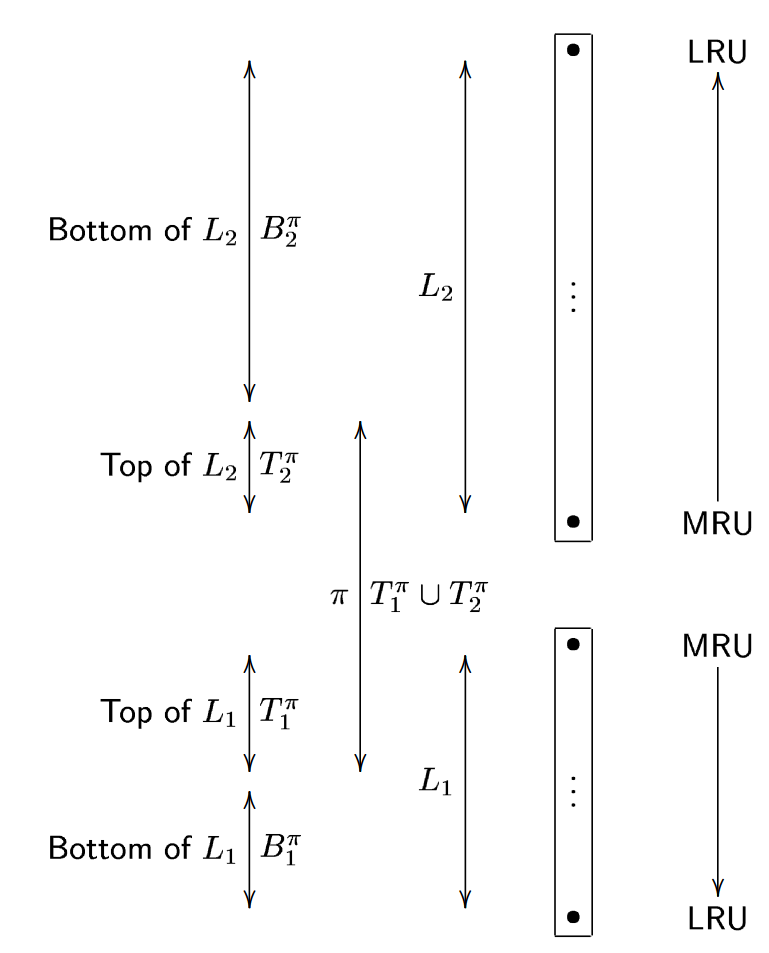
\includegraphics[width=8cm,height=9cm]{Figures/arc.PNG}
 \captionsetup[figure]{font=normalsize}
 \caption{General structure of generic cache replacement policy}
 \vspace{-0.5cm}
 \label{fig:arc}
\end{figure}


We now show brief explanation about ARC~\cite{arc}. Main difference between ARC and the other policies is that ARC adaptively changes its paramter. More specifically, the paramter of ARC is defined as the size of LRU/LFU portion within cache. We will show how it adaptively changes its size during runtime through Section A to C. 

\subsection{LRU and LFU}
 Many researchers attempted to make an algorithm that captures both recency and frequency. Since almost the whole workloads has both locality and frequency. So in order to the derive high hit ratio of the cache, For researchers, it was a fate to capture those properties together. However, all of them had critical drawbacks that they have to assign some value to their parameters in order to derive higher hit ratio, and it highly depends on the access pattern of certain workloads. Before describing ARC, We show a generic cache replacement policy which was used in ARC. Figure~\ref{fig:arc} shows the general structure of generic cache replacement policy. \\
 This policy ensures that following invariants will always hold:\\
 \vspace{-0.2cm}
 \begin{center}
 $ 0 \leq |L_1| + |L_2| \leq 2c$, $ 0 \leq |L_1| \leq c$, $0\leq |L_2| \leq 2c.$
 \end{center}

 
 Also, in below conditions A.1-5 hold for generic cache replacement policy.
 \vspace{0.2cm}
 \begin{itemize}
     \item A.1. The lists $T_1^\pi$ and $B_1^\pi$ are disjoint and, also, the lists $T_2^\pi$ and $B_2^\pi$ are disjoint, and 
     $L_1$ = $T_1^\pi$ $\cup$ $B_1^\pi$ and $L_2$ = $T_2^\pi$ $\cup$ $B_2^\pi$.
 \end{itemize}

\begin{itemize}
    \item A.2 If $|L_1 \cup L_2| < c$, then both $B_1^\pi$ and $B_2^\pi$ are empty.
\end{itemize}

\begin{itemize}
    \item A.3 If $|L_1 \cup L_2 | \geq c$, then, together $T_1^\pi$ and $T_2^\pi$ contain exactly c pages. 
\end{itemize}

\begin{itemize}
    \item A.4 Either $T_1^\pi$(resp. $T_2^\pi$) or $B_1^\pi$ (resp. $B_2^\pi$) is empty, or the LRU page in $T_1^\pi$ (resp. $T_2^\pi$) is more recent than the mRU page in $B_1^\pi$ (resp.$B_2^\pi$).
\end{itemize}

\begin{itemize}
    \item A.5 For all traces and at each time, $T_1^\pi \cup T_2^\pi$ will contain exactly those pages that would be maintained in cache by the policy $\pi(c)$.
\end{itemize}

 Key concept of this cache replacement policy is that $L_1$ holds pages that requested only once and $L_2$ holds pages that requested more than once. $|T_1 \cup T_2|$ is the actual cache and it keeps exactly the same size as cache size $c$. Compared to $T_1$ and $T_2$, $B_1$ and $B_2$ is used for the cache replacement management. i.e. ghost cache. In Figure~\ref{fig:arc}, the ghost cache size is set to $2c$.

\subsection{Ghost Cache}
In ARC, they maintain a larger cache directory than that is needed to support the underlying cache. Such directories are known as a shadow cache or as a ghost cache. Previously, ghost caches have been employed in a number of cache replacement algorithms. ARC uses this ghost cache for adaptively determine the size of $T_1$ and $T_2$, $B_1$ and $B_2$ respectively. 

\subsection{Adaptive Replacement Cache}


\begin{figure}[t]
 \centering
 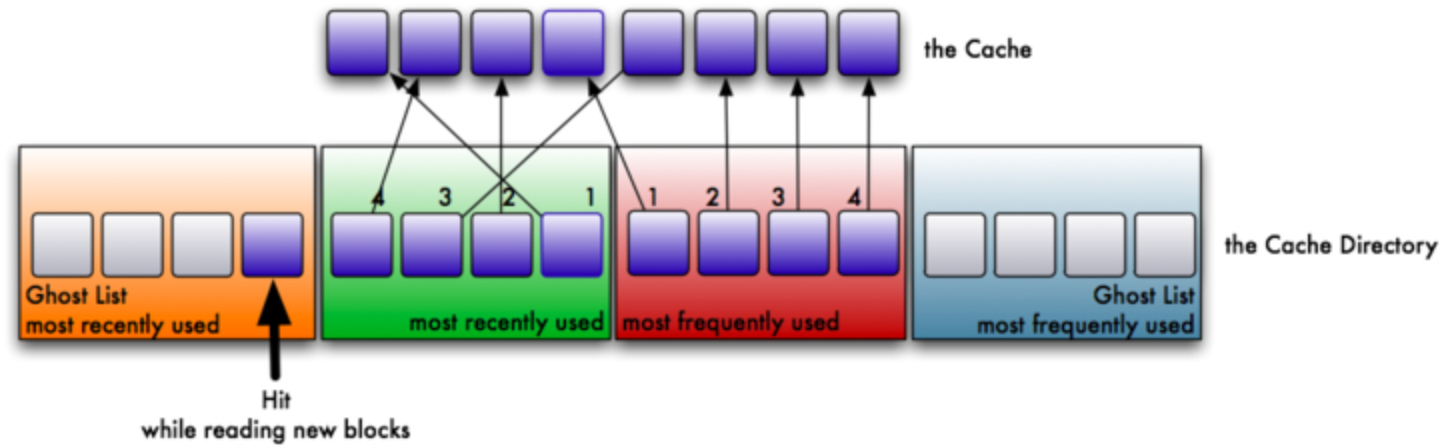
\includegraphics[width=9cm,height=5cm]{Figures/phantom_cache_hit.PNG}
 \captionsetup[figure]{font=normalsize}
 \caption{A situation that phantom hit occurs}
 \vspace{-0.5cm}
 \label{fig:phantom_hit}
\end{figure}


\begin{figure}[t]
 \centering
 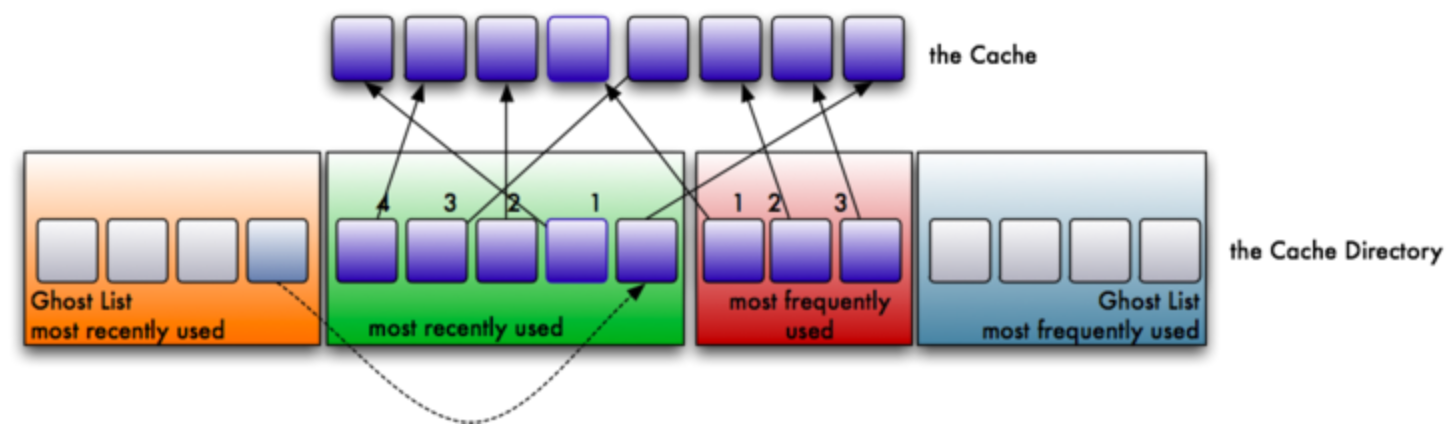
\includegraphics[width=9cm,height=5cm]{Figures/phantom_cache_hit_after.png}
 \captionsetup[figure]{font=normalsize}
 \caption{Adaptive resizing from ARC}
 \vspace{-0.5cm}
 \label{fig:phatom_hit_after}
\end{figure}


The main idea of ARC is quite simple. They maintain a ghost list i.e. $B_1$ and $B_2$.  when they encountered the cache miss, they treat it as a actual-miss or phantom-hit (i.e. hit on $B_1$ or $B_2$). So if phantom-hit occurs, then ARC adaptively resizes the portion of $T_1$(i.e. phantom hit on $B_1$) or $T_2$(phantom hit on $B_2$). This is not actually accurate because some exceptions exist. Note that we describe brief the concept of ARC so if interested in 
more detailed algorithm, See [Fig 4 in~\cite{arc}]. From Figure 2 and Figure 3, we can see the adaptive resizing of ARC, In Figure ~\ref{fig:phantom_hit}, We can see that actual cache size is 8. and ghost cache size is 16. Initial situation is same as following, $|T_1|=4, |B_1|=4, |T_2|=4, |B_2|=4$. Then phantom-hit occurs on $B_1$, So from that, ARC resizes the $|T_1|$ from $4$ to $5$, and $|T_2|$ from $4$ to $3$. $|B_1|$ and $|B_2|$ has same value in Figure 2 and 3. Note that this is a example for explaining ARC and it is not exactly same as ARC(i.e. a variant from ZFS-ARC) but the main idea(i.e. adaptive replacement) is same. Actually, various cases happen when a phantom-hit or actual miss occurs. See [Fig 4 in ~\cite{arc}]. 

